\section{Claw-SWE-Bench}
\label{sec:claw_swe_bench}

The first question in this paper is whether a general-purpose agent such as OpenClaw can enter a SWE-bench-style evaluation of real coding tasks. To make this question experimentally testable, we first specify the SWE-bench~\cite{jimenez_swebench_2024} scoring contract. Given the \texttt{problem\_statement}, target \texttt{repo}, and \texttt{base\_commit} for a real GitHub issue, a system must submit a diff patch that can be applied to the repository checkout. The official evaluation harness does not read an interaction trace or a final natural-language answer. It reads a prediction file in which each instance contains at least \texttt{instance\_id}, \texttt{model\_name\_or\_path}, and a string-valued \texttt{model\_patch}. The evaluator then prepares the repository in the Docker evaluation environment for that instance, applies the patch to the checkout under \texttt{/testbed}, and runs repository-level tests to determine whether the instance is resolved. In short, the core SWE-bench interface is an evaluator-facing patch prediction, not a generic agent session.

Coding harnesses such as SWE-agent~\cite{swe_agent} are designed around this contract. OpenClaw, by contrast, is normally run as a more general agent interaction and therefore cannot be treated as a SWE-bench evaluation target without adaptation. First, the SWE-bench Docker image is primarily a reproducible target-repository, dependency, and test environment; it does not itself provide the agent lifecycle, tool configuration, API access, session state, or workspace management required by OpenClaw. These runtime dependencies and state must be brought inside a controlled container boundary while ensuring that the agent's actual code edits occur in \texttt{/testbed}. Second, general-purpose agents often signal completion through final text, structured messages, or internal logs, whereas the SWE-bench evaluator reads only the \texttt{model\_patch} field. Explanatory answers are not directly scorable. Third, a general agent can create session files, metadata, caches, or other non-solution artifacts during execution; if these enter \texttt{git diff}, they contaminate the patch submitted to the evaluator.

These limitations do not imply that OpenClaw lacks coding ability. They imply that native OpenClaw cannot directly enter the SWE-bench scoring pipeline. The premise we first challenge is that SWE-bench-style coding tasks must be solved only by purpose-built coding harnesses. General-purpose agents can participate in real issue resolution if an adapter constrains their behavior to concrete repository edits and converts the final repository state into an evaluator-readable patch. Once this access problem is solved, the next step is to define a unified evaluation standard that compares the coding ability and run cost of different claws or harnesses under the same tasks, budgets, and scoring pipeline.

We therefore propose \textsc{Claw-SWE-Bench}, a multilingual SWE-style benchmark and execution protocol for evaluating coding-agent harnesses. It combines 350 real GitHub issue-resolution tasks across 8 programming languages with a unified adapter layer, allowing heterogeneous ``claws'' -- agent harnesses that wrap LLMs into autonomous coding systems -- to run under the same evaluation protocol.

\textsc{Claw-SWE-Bench} achieves this in two layers. The first layer is the adapter: it connects the native execution style of a general or specialized harness to the repository-editing and patch-prediction process required by SWE-bench, making these systems eligible for the same class of coding tasks. The second layer is a shared orchestrator: it fixes the task set, repository state, task prompt, Docker runtime, outer budget, patch extraction, prediction format, and downstream SWE-bench evaluation, elevating the harness from an incidental implementation detail to an experimental variable. Under this control, differences in Pass@1, wall-clock duration, and turn traces can be attributed to model or harness dimensions rather than to inconsistent evaluation protocols. The rest of this section describes the workload source, adapter protocol, and standardized execution pipeline.

\begin{figure}[t]
  \centering
  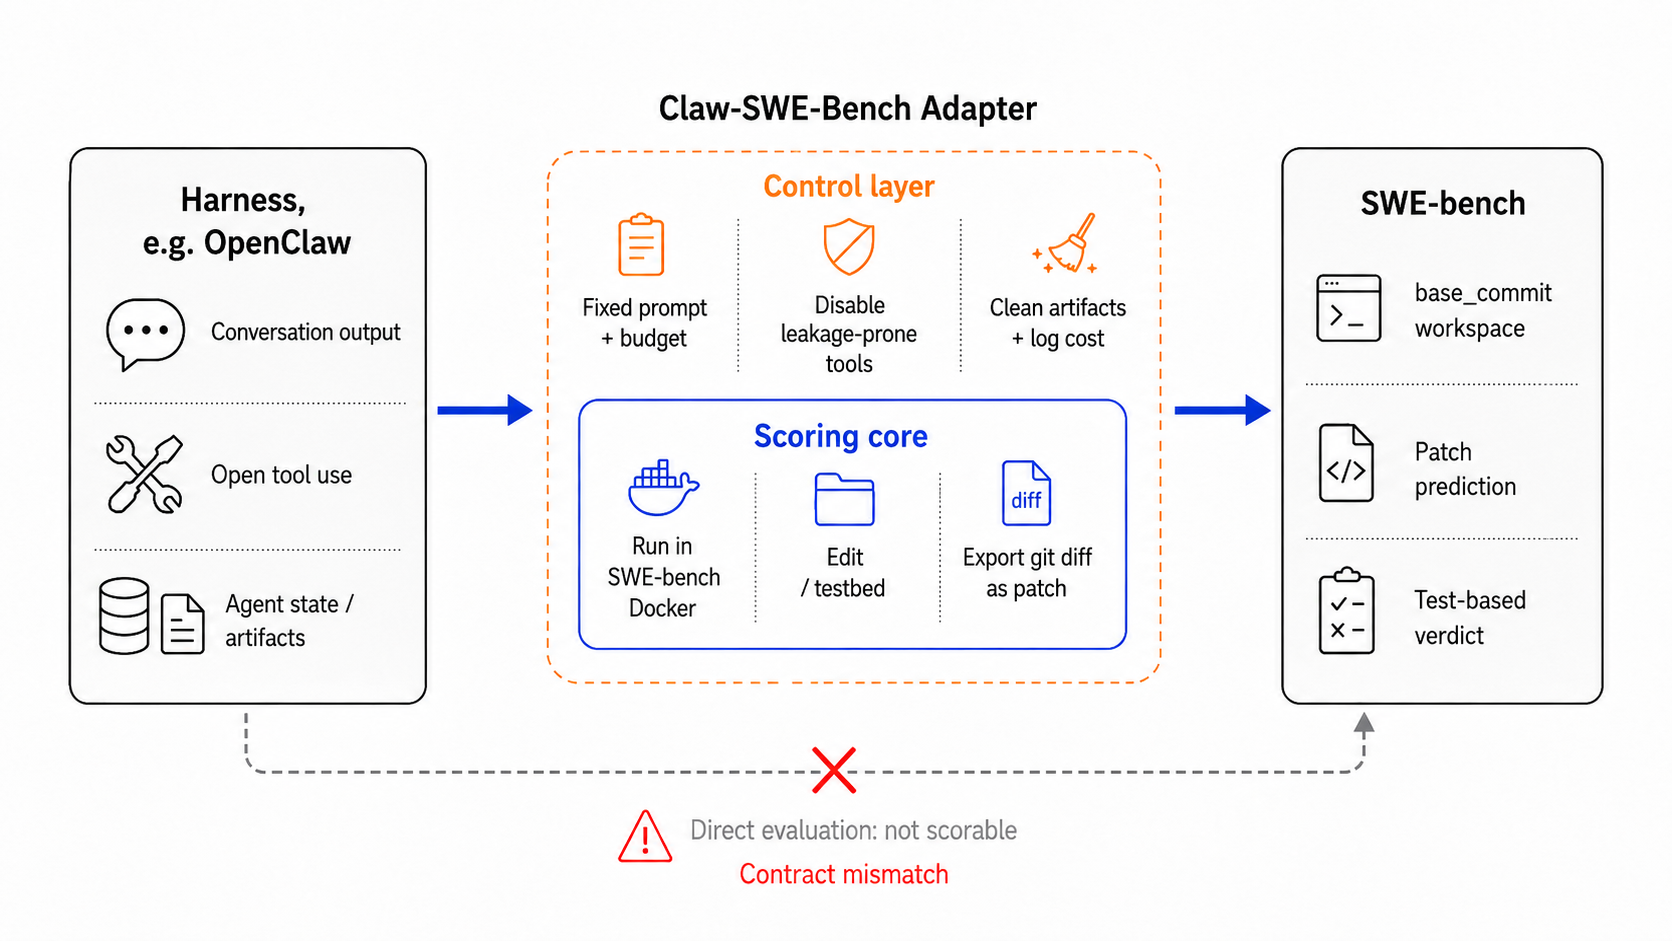
\includegraphics[width=0.9\linewidth]{figs/C_figure3.png}
  \vspace{-3mm}
  \caption{\textbf{Contract mismatch between OpenClaw-style harnesses and SWE-bench.}
The adapter converts a general agent interaction into a SWE-bench-scored patch prediction, while outer controls ensure fairness, comparability, and traceable cost.}
  % \vspace{-5mm}
  \label{fig:framework_pipeline}
\end{figure}

\subsection{Workload Source and Composition}
\label{sec:benchmark_workload}

The full \textsc{Claw-SWE-Bench} workload is built from two upstream SWE-bench-derived sources. SWE-bench-Multilingual~\cite{swe_smith} contributes 300 non-Python instances covering Java, Go, Rust, JavaScript/TypeScript, C/C++, Ruby, and PHP. SWE-bench-Verified-Mini~\cite{swebench_verified_mini} contributes 50 human-validated Python instances. Together, the full benchmark contains 350 real GitHub issue-resolution tasks across 8 programming languages and 43 repositories.

Each instance preserves the upstream SWE-bench task format and evaluation assets, including \texttt{problem\_statement}, \texttt{repo}, \texttt{base\_commit}, the corresponding Docker evaluation image, and the repository-level tests used for scoring. This combination serves two purposes. First, the benchmark remains compatible with SWE-bench's patch-based evaluation. Second, multilingual tasks and human-validated Python tasks jointly provide broader real-software-engineering coverage, so harness comparisons are not limited to one language or one upstream subset. All model--harness combinations are run on the same 350 instances, allowing resolved-rate and cost differences to be interpreted under a fixed workload.

\subsection{Adapter Protocol}
\label{sec:adapter_protocol}

The adapter protocol is the first layer of \textsc{Claw-SWE-Bench}. It does not require different harnesses to use the same internal agent loop; instead, it standardizes the interface between a harness and the benchmark lifecycle. Each supported harness implements the same abstract methods: \texttt{create\_agent}, \texttt{send\_task}, \texttt{backup\_session}, \texttt{delete\_agent}, and \texttt{get\_docker\_args}. The shared orchestrator drives a run only through these methods, without needing to know which harness is underneath. This design decouples the benchmark lifecycle from agent implementation: container management, prompt instantiation, patch collection, prediction writing, metadata recording, resume support, and evaluation are implemented by the benchmark layer, while each harness adapter only connects its agent to that lifecycle and provides the code needed to drive the agent inside the container.

At runtime, the shared orchestrator enforces the access boundary shown in Figure~\ref{fig:framework_pipeline}. Container startup, repository reset, prompt instantiation, patch collection, prediction writing, metadata recording, and evaluation are handled uniformly by the benchmark layer. The adapter provides harness-specific hooks to create or configure the agent, dispatch the instantiated task, save run artifacts, and clean harness state. This boundary is deliberate: the benchmark layer owns the task-facing environment and evaluator-facing patch format, while the internal agent loop remains part of the harness being studied.

Crucially, candidate patches are collected from repository state rather than parsed from an agent's final message. An agent expresses a solution only by editing files in the repository. This makes the output contract independent of whether the harness natively produces JSON, plain text, a final narrative response, or no structured response at all.

All harnesses are launched through the same command-line entry point, \texttt{run\_infer.py}. The evaluator specifies the harness name, dataset configuration, model identifier, run identifier, timeout, worker count, and optional instance filters. Dataset metadata is loaded from configured SWE-bench sources, and each instance is represented by the fields required by the protocol: \texttt{instance\_id}, \texttt{repo}, \texttt{base\_commit}, and \texttt{problem\_statement}. A harness registry maps string IDs (\texttt{openclaw}, \texttt{hermes}, \texttt{nanobot}, \texttt{zeroclaw}, and \texttt{generic}) to adapter classes. Adding a new claw only requires implementing the adapter interface and registering it in the harness map; the dataset loader, Docker workspace manager, prompt builder, patch collector, prediction writer, and evaluator remain unchanged.

\subsection{Standardized Execution Pipeline}
\label{sec:exec_pipeline}

The adapter determines whether heterogeneous harnesses can enter a common evaluation protocol. Outside that boundary, \textsc{Claw-SWE-Bench} further fixes the evaluation-stack components that would otherwise confound harness comparisons.

\textbf{Runtime and workspace.}
Each task runs inside its corresponding SWE-bench evaluation Docker image, with the repository reset to the instance's \texttt{base\_commit} and mounted at \texttt{/testbed}. For the seven non-Python languages from SWE-bench-Multilingual, we also handle future-commit visibility during workspace preparation. While inspecting the containers, we found that some images still exposed Git commits after \texttt{base\_commit}; if left unchanged, an agent could inspect future fixes through \texttt{git log} or \texttt{git show}, which is incompatible with the patch-based evaluation contract. The runner therefore removes reachable future commits so that the agent can only read, edit, and run code within the history boundary of the issue. All harnesses share the same outer budget: a 3600-second wall-clock timeout, one run per instance, and fixed worker concurrency. Harness-specific dependencies can be supplied through Docker arguments or bind mounts, but the repository state, evaluation image, and outer budget perceived by the agent are fixed. These budget controls prevent longer exploration time from being mistaken for stronger harness design and make cost metrics comparable across harnesses. Because different harnesses define a ``turn'' differently, wall-clock duration is the primary comparable resource metric; turn count is treated as a diagnostic trace. Token statistics are available for some harnesses but not exposed uniformly by all systems, so they are not the sole cross-harness metric.

\textbf{Prompt instantiation.}
Every instance is instantiated from the same task-prompt template. The prompt includes the problem statement and base commit, instructs the agent to work in \texttt{/testbed}, forbids \texttt{git add} and \texttt{git commit}, and asks the agent not to modify test files. Thus the task-facing input message is held fixed across harnesses. The protocol does not attempt to standardize a harness's internal system prompt, tool schema, parser hints, memory strategy, or stopping rule; these remain part of harness design and therefore part of the experimental variable.

\textbf{Patch and scoring contract.}
Candidate solutions are collected from repository state rather than parsed from the agent's final response. After a harness terminates, times out, or returns an error, the runner computes the diff against the base commit, removes known non-solution artifacts, and writes a SWE-bench-compatible prediction. This centralized patch-submission process allows heterogeneous harnesses to be compared even when their native outputs differ: JSON, plain text, natural-language summaries, and missing structured responses are all reduced to the same evaluator-facing patch format. Evaluation is then performed by the official SWE-bench harness.

To separate ``placing OpenClaw inside Docker'' from ``reliably satisfying the SWE-bench scoring contract,'' we also define a minimal \emph{bare adapter} as a diagnostic baseline. The bare adapter provides only minimal integration: it enters the corresponding Docker workspace for each instance, sends the issue description to OpenClaw, and disables network retrieval that would clearly violate fairness. It does not perform full workspace alignment, future-commit cleanup, shared phase prompting, Git-based patch extraction, or patch cleaning; instead, it asks the model to output a unified diff directly in the final response. By contrast, the full adapter used in the main experiments requires the agent to edit files under \texttt{/testbed}, after which the runner exports \texttt{model\_patch} from the final repository state. This comparison tests the necessity of the adapter, not the attribution of individual adapter components.
